\documentclass[dutch, a4paper, 11pt]{article}
\usepackage[utf8]{inputenc}
\usepackage[english]{babel}
\usepackage{pgfplots}
\pgfplotsset{width=10cm,compat=1.9}

%Margins 
\usepackage[a4paper, left=1.27cm,top=1.27cm,right =1.27cm, bottom = 1.4cm]{geometry}

%Load packages
%Algemene packages
\usepackage{babel}
\usepackage{slantsc}
\usepackage{array}
\renewcommand{\arraystretch}{2}
\usepackage{multicol}
\usepackage{multirow}
\usepackage{amsmath}
\usepackage{amsfonts}
\usepackage{booktabs}

%Opsommingen
\usepackage{enumerate}


%Afbeeldingen
\usepackage{graphicx}
\usepackage{wrapfig}

%Gekleurde tekstboxen 
\usepackage[most]{tcolorbox}

%Stop indent
\setlength{\parindent}{0pt}

%Font
\usepackage{cmbright}
\usepackage[OT1]{fontenc}

%Headers and footers
\usepackage{fancyhdr}

\pagestyle{fancy}
\fancyhf{}
\renewcommand{\headrulewidth}{0pt}
\renewcommand{\footrulewidth}{0pt}
\fancyhead[LE,RO]{}
\fancyhead[RE,LO]{}

%Logo in footer
\usepackage{lastpage}
\lfoot{}
\cfoot{\vspace{-5mm} \thepage}
\rfoot{}

%Voorbeeldtekst
\usepackage{lipsum}

%Meerdere kolommen
\usepackage{multicol}
\setlength{\columnsep}{1cm}

%Whitespace na section
\usepackage[compact]{titlesec}  
\titlespacing{\section}{0pt}{2pt}{0pt}

%Tekst kleur
\usepackage{xcolor}

%Nieuwe kleur
%\definecolor{ugent_blue}{rgb}{0.04706, 0.13725, 0.26667}
\definecolor{ugent_blue}{RGB}{30, 100, 200}

%Nummering sections
\renewcommand\thesection{\arabic{section}}
\renewcommand\thesubsection{\thesection.\arabic{subsection}}

%Lay-out hoofdingen
\titleformat*{\section}{\bfseries \normalfont}
\usepackage{sectsty}
\sectionfont{\color{ugent_blue}}
\titlespacing\section{0pt}{10pt plus 4pt minus 4pt}{0pt plus 2pt minus 2pt}

\raggedbottom


%other shit that may be useful
\usepackage{multicol,caption}
\usepackage{mathtools}
\raggedbottom
\newcommand{\HRule}{\hrule}
\abovedisplayskip0pt
\renewcommand{\arraystretch}{1.5}
\newcolumntype{M}[1]{>{\centering\arraybackslash}m{#1}}
\usepackage{lscape}
\newenvironment{Figure}
  {\par\medskip\noindent\minipage{\linewidth}}
  {\endminipage\par\medskip}
\usepackage{float}
\usepackage{hyperref}
\newcommand\myfigure[1]{%
\medskip\noindent\begin{minipage}{\columnwidth}
\centering%
#1%
%figure,caption, and label go here
\end{minipage}\medskip}
\usepackage{caption}
\usepackage{subcaption}
\usepackage{tabularx}
\usepackage{enumerate}
\usepackage{enumitem}

\raggedbottom
\raggedcolumns


\graphicspath{{figures/}}

%units
\newcommand{\MW}{\frac{\text{g}}{\text{mol}}}
\newcommand{\g}{\text{g}}
\newcommand{\ml}{\text{ml}}
\newcommand{\density}{\frac{\text{g}}{\text{ml}}}
\newcommand{\mole}{\text{mol}}
%symbols
\newcommand{\mathtext}[2][]{\text{#2}_{\text{#1}}}

\begin{document}

%Load heading of document
%ugent color
{\color{ugent_blue} \hrule\hrule\hrule}

\vspace*{-0.43mm}
\colorbox{ugent_blue}{\color{white} \bf Report Biomechanics}\\

\noindent\begin{minipage}{0.7\textwidth}% adapt widths of minipages to your needs
{\LARGE \bf \color{ugent_blue} Clinical Movement Analysis Lab Assignment 2022}\\[2mm]

%
{\large Vincent Belpaire}\\
{Supervisor: Prof. Malcolm Forward}\\


{\small University of Ghent}\\
{\small Faculty of Engineering and Architecture}\\
{\small Bachelor of Science: Biomedical Engineering}\\
\end{minipage}%
\hfill%
\begin{minipage}{0.3\textwidth}
\vspace{-2.2cm}
\begin{center}

\includegraphics[width=\linewidth]{ugent_logo}
\end{center}
\end{minipage}\\

\section{Question 1: GelMA}

\begin{figure}[H]
    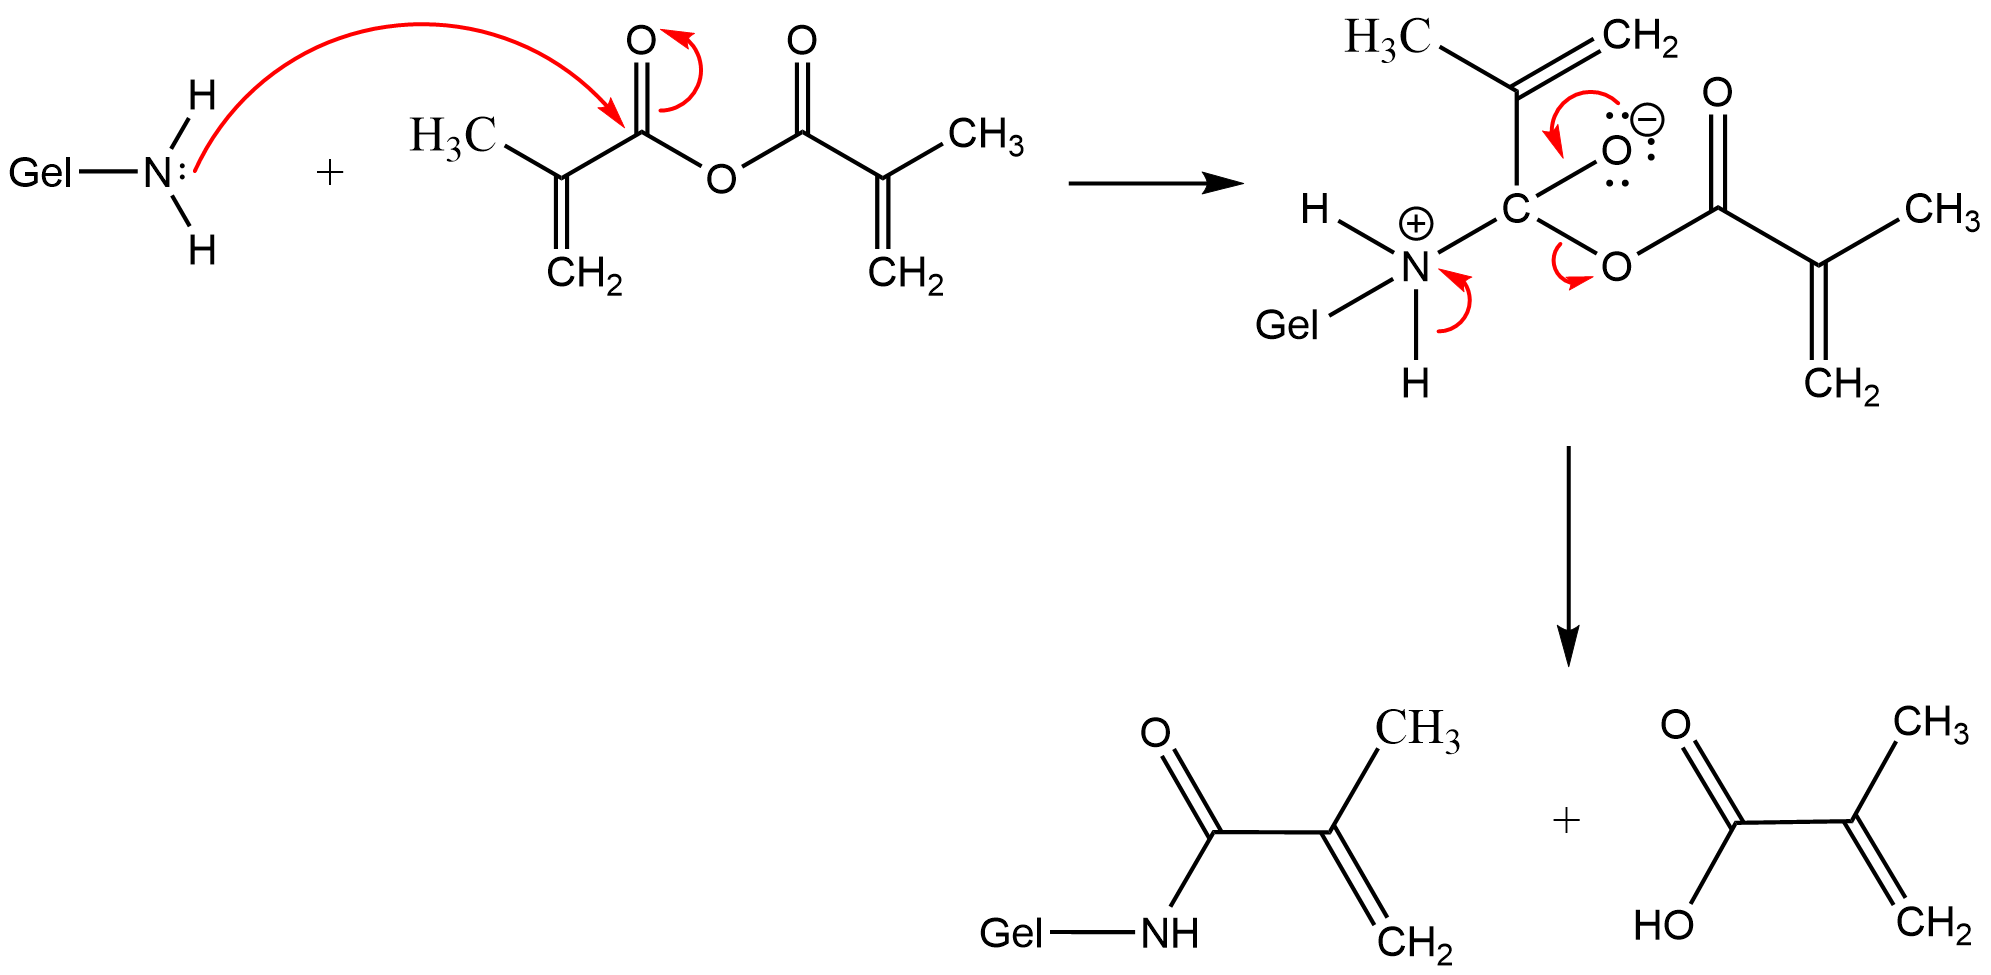
\includegraphics[width=\textwidth]{gelMA.png}
    \caption{Methacrylation of gelatin}
    \label{fig:gelMA}
\end{figure}

\subsection{Question 2: Rheology}

The different DS values for the differennt batches are calculated as

\begin{equation}
    DS = \frac{n_{\text{methacrylamide}}}{n_{\text{amine}}},
    \label{eq:DS}
\end{equation}

in which $n_{\text{amine}} = 0.385\unit{mmol}$ and

\begin{equation}
    n_{\text{methacrylamide}} = \frac{I(5.5\unit{ppm})+I(5.75\unit{ppm})}{2\cdot k},
    \label{eq:nMA}
\end{equation}

where $k$ is calculated as

\begin{equation}
    k = \frac{I(1\unit{ppm})}{6\cdot n_{\text{VLI}}},
    \label{eq:j}
\end{equation}

with $n_{\text{VLI}}=0.64\unit{mmol}$. All the data, from the NMR spectra on UFORA, and the calculated values are found in table \ref{tab:researcher1}.

\begin{table}[H]
    \centering
    \begin{tabular}{ccccccc}
      batch & $I(1\unit{ppm})$ & $I(5.5\unit{ppm})$ & $I(5.75\unit{ppm})$ & $k$ [1/mmol]& $n_{\text{methacrylamide}}$ [mmol] & DS [\%]\\
      \hline
      A & 142871.9 & 4918.98 & 4790.75 & 37206.22 & 0.130 & 34\\
      B & 166032.1 & 12362.5 & 12140.48 & 43237.53 & 0.283 & 74\\
      C & 114480.1 & 10858.83 & 1162.68 & 29812.83 & 0.369 & 96\\
    \end{tabular}
    \caption{DS values for the differennt batches}
    \label{tab:researcher1}
\end{table}

\begin{figure}[H]
    \centering
    \begin{subfigure}[b]{0.45\textwidth}
    \centering
    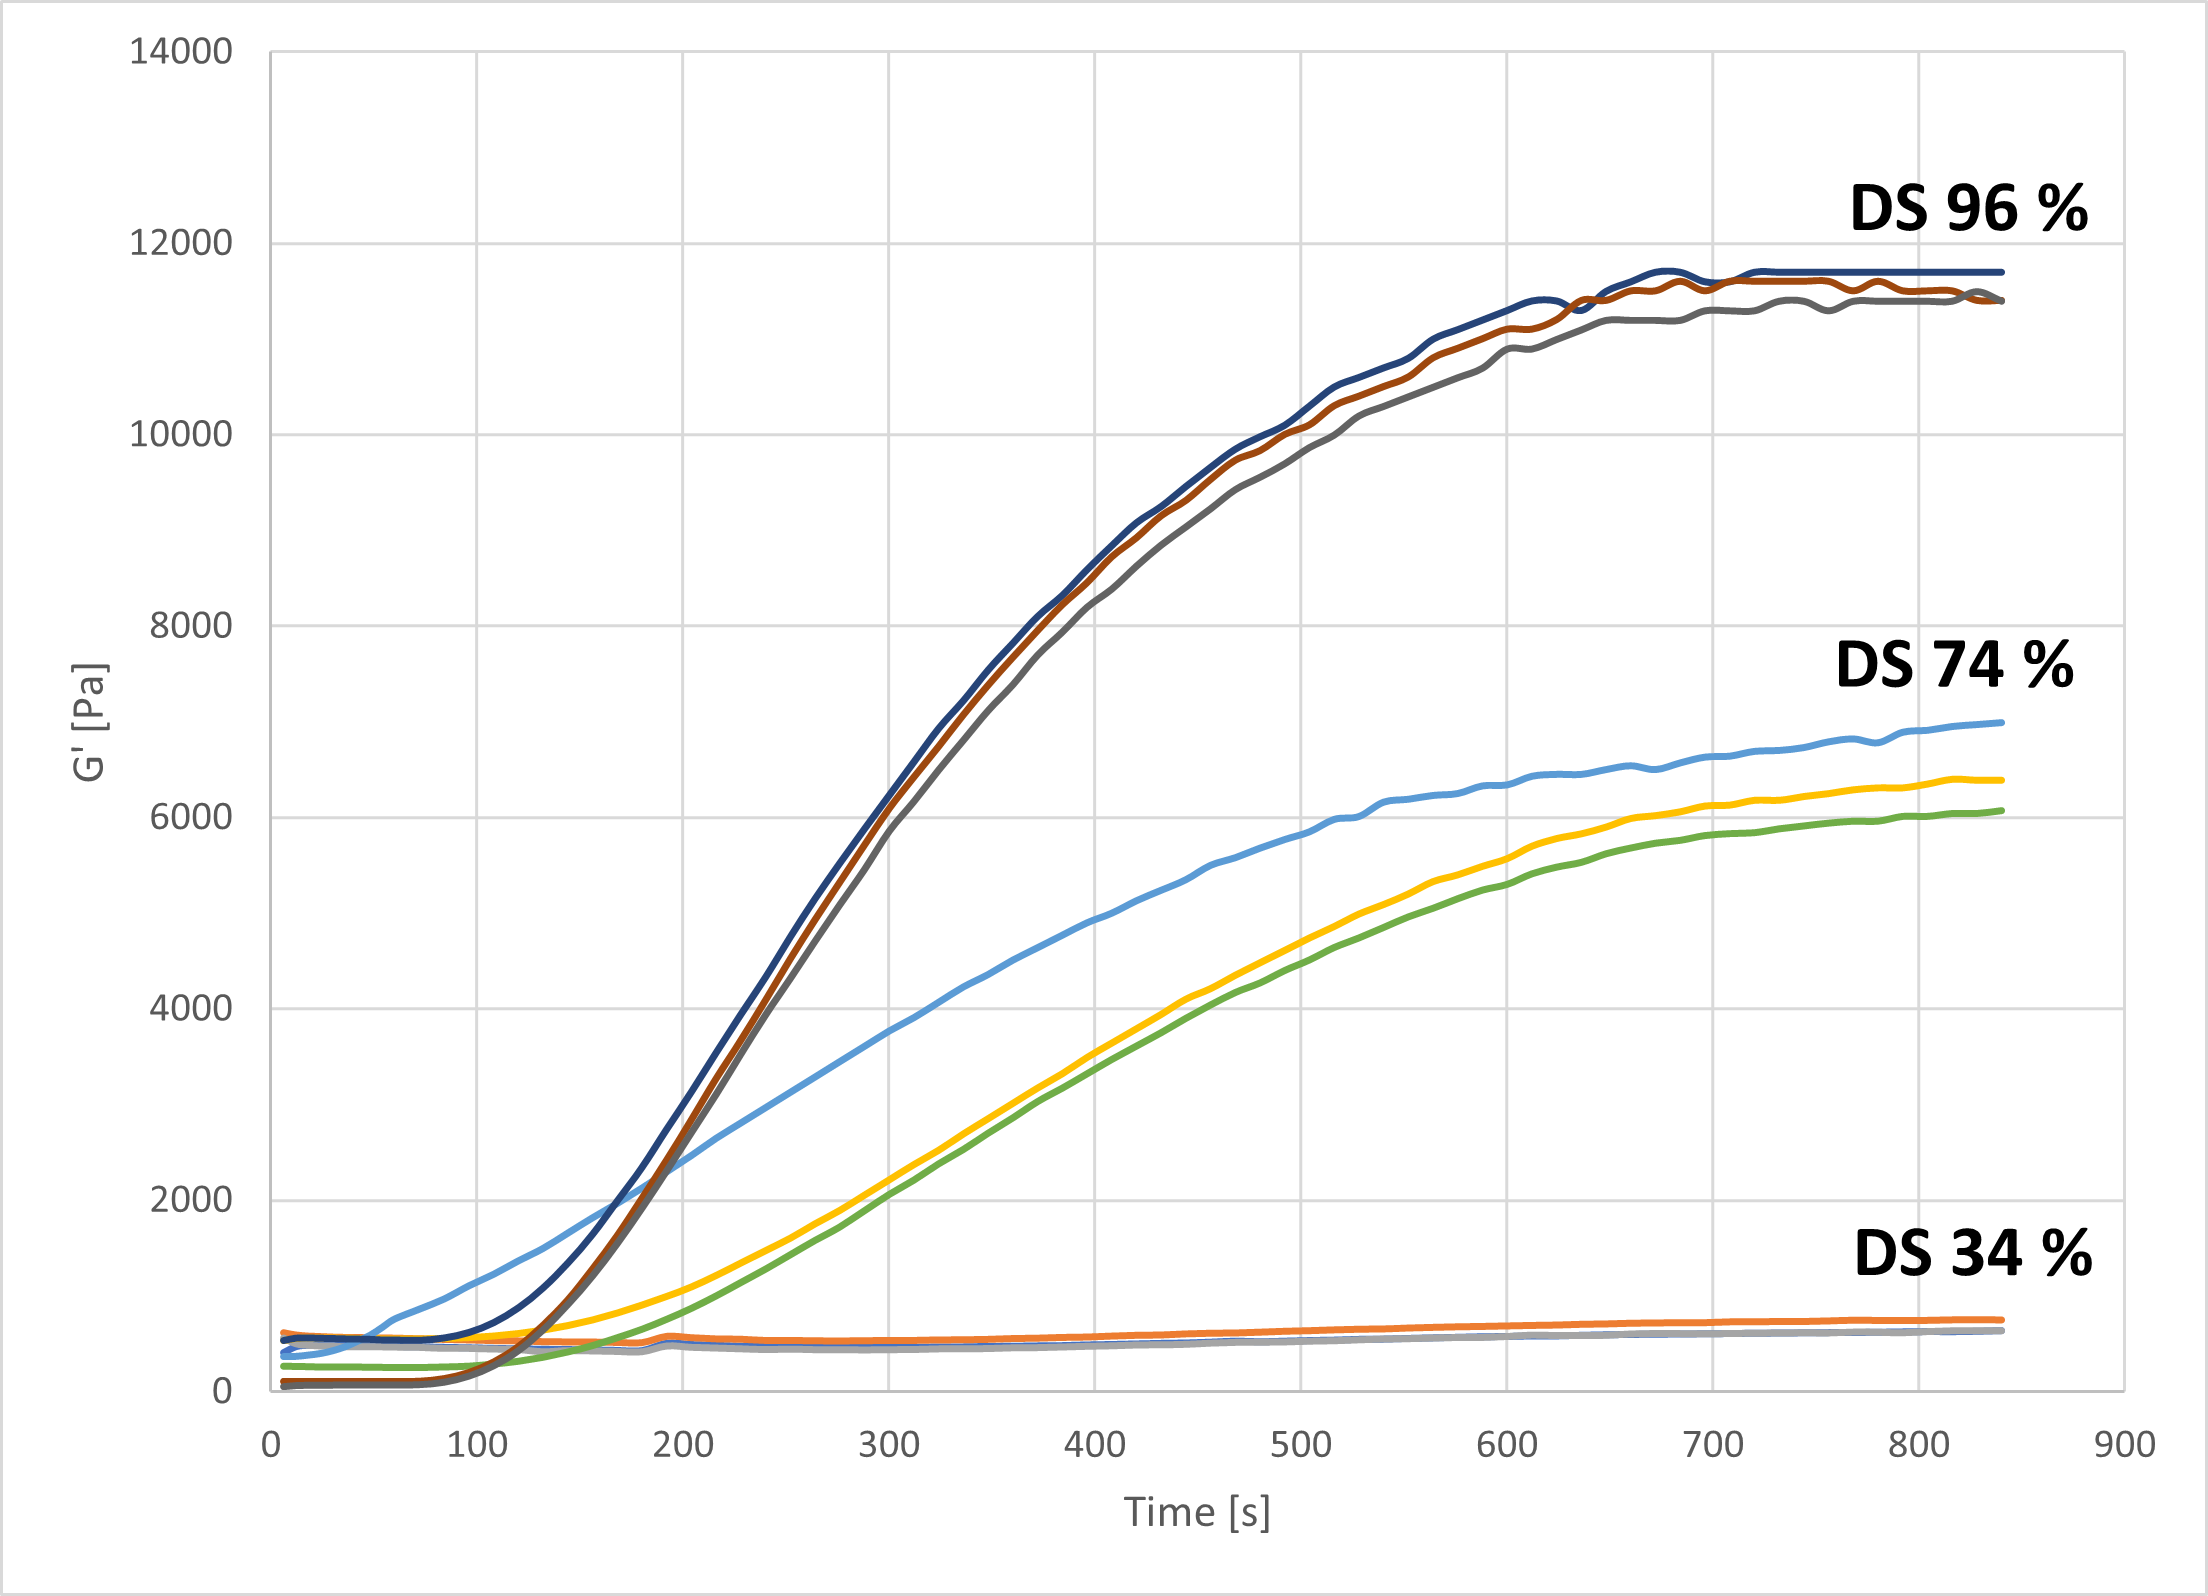
\includegraphics[width=\textwidth]{in_situ_UV_crosslinking_person1.png}
    \end{subfigure}
    \begin{subfigure}[b]{0.45\textwidth}
    \centering
    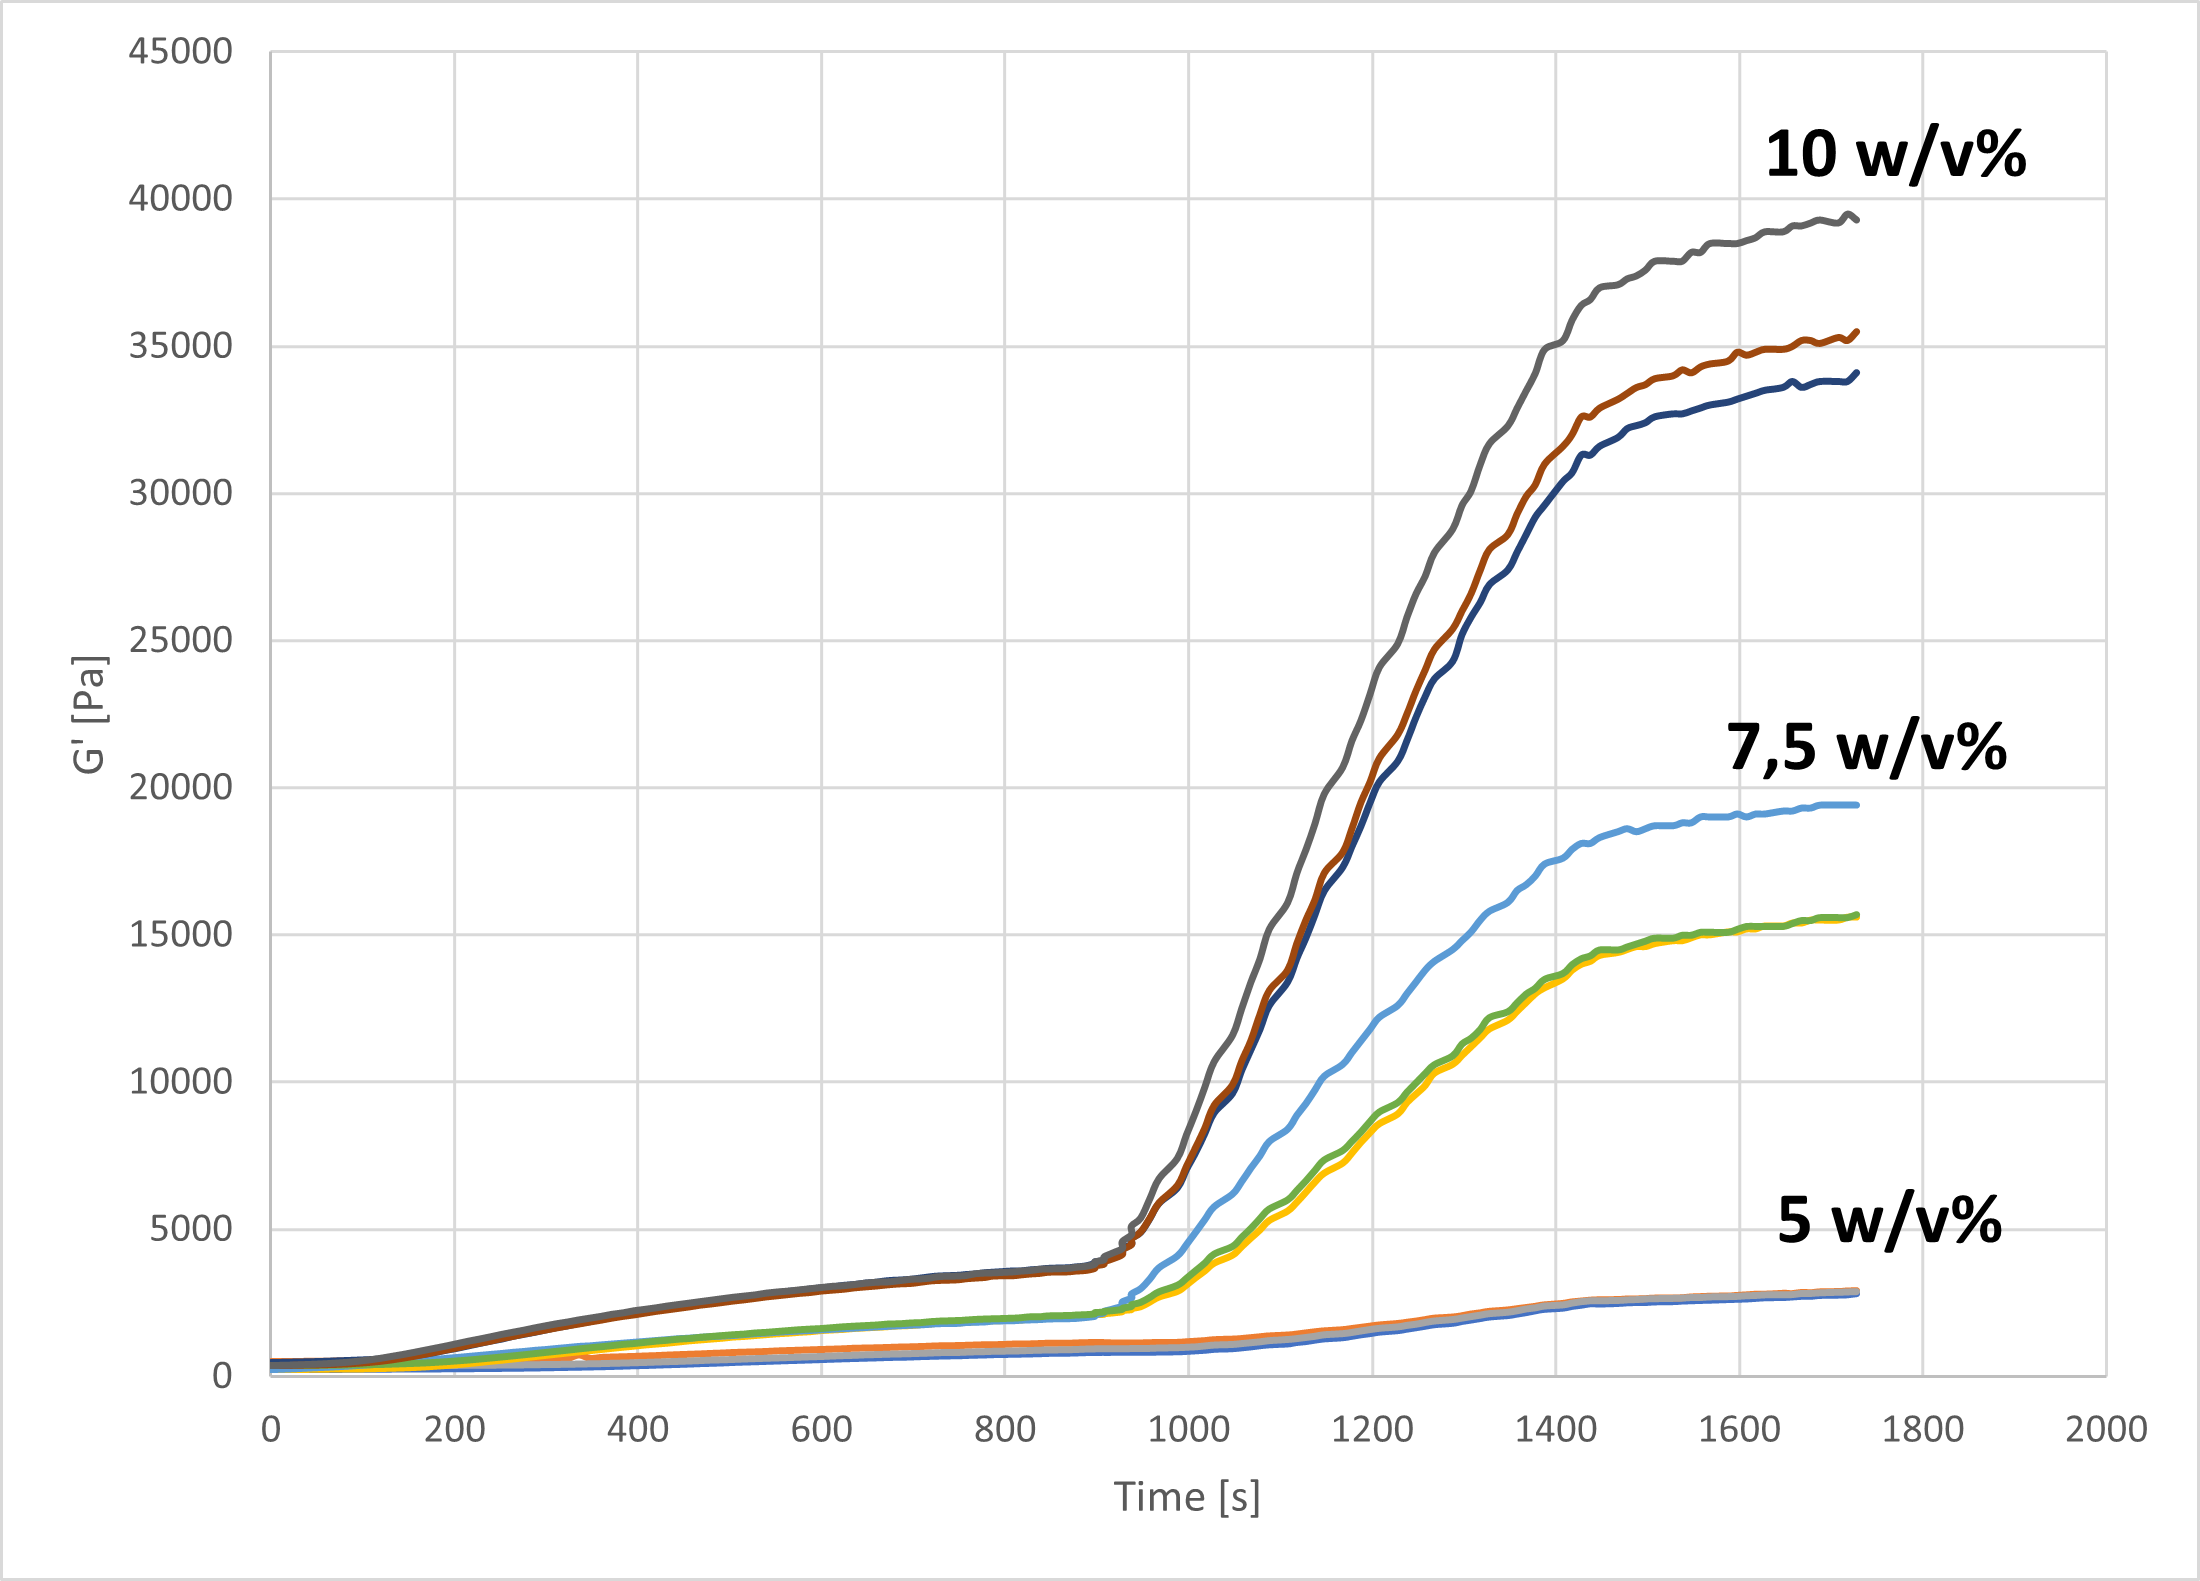
\includegraphics[width=\textwidth]{in_situ_UV_crosslinking_person2.png}
    \end{subfigure}
    \caption{Rheological in-situ UV-crosslinking with varying DS (right) and varying w/v\% (left)}
    \label{fig:rheo}
\end{figure}

Figure 2 displays rheological data from different researchers. The storage modulus $G'$ increases with increasing DS as well as with increasing w/v\%. $G'$ is a parameter that relates to the elasticity of the material obtained, indicating the amount of energy stored in the material due to deformation. Higher $G'$ values indicate that the material is stiff, while lower values indicate a more elastic behavior. In this rheology setup, gelMA is subjected to oscillating stress or strain while being irradiated by UV light, causing it to crosslink. $G'$ is measured during this crosslinking process, with more crosslinks implying a stronger force holding the material structure together. Higher DS values or higher concentrations of gelMA can induce more crosslinks. This theory corresponds perfectly with the obtained data. Furthermore, a steeper increase in $G'$ indicates a higher crosslinking speed. Once most of the gelMA is crosslinked, $G'$ reaches a plateau value.

A difference between the two measurements is apparent. The data from the left graph (researcher 1) was collected over a smaller time interval, and the maximum $G'$ is much lower compared to that of researcher 2, as both used batch C at 10 w/v\%. One possibility for this difference in measurement could be the amount of photo-initiator added to the gelMA. 



\section{Question 3: Texturometry}

Two differences in the mechanical testing method:
\begin{itemize}
    \item[1.] Rheology measures the flow and deformation of materials under applied stress or strain, while texturometry 
    measures the mechanical properties of materials under compression, tension, or shearing forces.
    \item[2.] Rheology tests are typically performed using a rheometer, which applies precise controlled shear or tensile 
    stresses to the sample and measures the resulting deformation or stress response. Texturometry tests, on the other 
    hand, are performed using a texture analyzer, which applies a compressive, tensile, or shearing force to the sample and measures the resulting deformation or force response.
\end{itemize}

Next, two texturometry tests were performed by two researchers. Table \ref{tab:inverted-mechanical-test-results} and \ref{tab:inverted-mechanical-test-results-10wv} are results of a texture profile analysis (TPA) from researcher 1. 
Compairing the hardness, the ability to resist deformation, and springiness, the ability to recover to the original shape after compression, between the two tables indicate that higher w/v\% values results in a stiffer/harder material with a better ability to recover to its original shape after compression. 
If the DS of the material would br  

\begin{table}[H]
    \centering
    \begin{tabular}{c|ccc}
    \hline
    & Sample 1 & Sample 2 & Sample 3 \\ \hline
    Hardness1 [N] & 0.035167098 & 0.043005662 & 0.04099971 \\ 
    Hardness2 [N] & 0.030627189 & 0.032652594 & 0.040604329 \\ 
    Area1 [Nmm] & 0.003338952 & 0.002307124 & 0.003828073 \\ 
    Area2 [Nmm] & 0.001615961 & 0.000898191 & 0.002239604 \\ 
    Cohesiveness & 0.483972601 & 0.389311989 & 0.585047474 \\ 
    Springiness [mm] & 0.282010363 & 0.218791648 & 0.270347203 \\ 
    Springiness Index & 0.531212397 & 0.402065399 & 0.544778107 \\ 
    Gumminess [N] & 0.017019912 & 0.01674262 & 0.023986777 \\ 
    Chewiness [Nm] & 4.79979E-06 & 3.66315E-06 & 6.48476E-06 \\
    \end{tabular}
    \caption{TPA results - 5 w/v\%}
    \label{tab:inverted-mechanical-test-results}
\end{table}

\begin{table}[H]
    \centering
    \begin{tabular}{c|ccc}
    \hline
    & Sample 1 & Sample 2 & Sample 3 \\ \hline
    Hardness1 [N] & 0.067449574 & 0.06582288 & 0.072415185 \\ 
    Hardness2 [N] & 0.06262254 & 0.064647785 & 0.067325579 \\ 
    Area1 [Nmm] & 0.007224188 & 0.006074186 & 0.008424538 \\ 
    Area2 [Nmm] & 0.005469138 & 0.004678299 & 0.005826683 \\ 
    Cohesiveness & 0.757059224 & 0.770193572 & 0.691632352 \\ 
    Springiness [mm] & 0.465056416 & 0.38483355 & 0.420807332 \\ 
    Springiness Index & 0.889844319 & 0.767740421 & 0.767942963 \\ 
    Gumminess [N] & 0.051063322 & 0.050696359 & 0.050084685 \\ 
    Chewiness [Nm] & 2.37473E-05 & 1.95097E-05 & 2.1076E-05 \\
    \end{tabular}
    \caption{TPA results - 10 w/v\%}
    \label{tab:inverted-mechanical-test-results-10wv}
    \end{table}

\subsection{Question 4: Processing}

2-Photon Polymerization (2PP) is a suitable technique to replace traditional photolithography when speed is not a critical factor. In 2PP, two photons are absorbed by the photo-initiator, resulting in a highly localized crosslinking reaction that yields high resolution. Additionally, 2PP allows for precise control over process parameters, such as laser power, scanning speed, and exposure time. 

\end{document}
